\documentclass[journal,twoside,web]{ieeecolor}

\usepackage{generic}
\usepackage{cite}

\usepackage{amsmath}
\usepackage{amssymb}
\usepackage{amsfonts}
\usepackage{mathtools}
\usepackage{bm}

\usepackage{graphicx}
\usepackage{booktabs}
\usepackage{makecell}
\usepackage{multirow}
\usepackage{multicol}

\usepackage{algorithm}
\usepackage{algpseudocode}

\usepackage{textcomp}
\usepackage{pifont}
\usepackage{soul}
\usepackage{url}
\usepackage[switch]{lineno}
\usepackage[hidelinks]{hyperref}

\newtheorem{theorem}{Theorem}

\def\BibTeX{{\rm B\kern-.05em{\sc i\kern-.025em b}\kern-.08em
    T\kern-.1667em\lower.7ex\hbox{E}\kern-.125emX}}
\markboth{\hskip22pc IEEE JOURNAL OF BIOMEDICAL AND HEALTH INFORMATICS}
{Xiong \MakeLowercase{\textit{et al.}}: Transport-Coupled Bayesian Flows for Molecular Graph Generation}
\begin{document}
\title{Transport-Coupled Bayesian Flows for Molecular Graph Generation}
\author{
    Yida Xiong$^{1,2}$, Jiameng Chen$^1$, Kun Li$^1$, Hongzhi Zhang$^1$, Xiantao Cai$^1$, Jia Wu$^3$, Lei Lei$^{4,\ast}$, Wenbin Hu$^{1,2,5\ast}$
    \thanks{$^1$ School of Computer Science, Wuhan University, China}
    \thanks{$^2$ Hubei Jiangxia Laboratory, China}
    \thanks{$^3$ Department of Computing, Macquarie University, Australia}
    \thanks{$^4$ Institute of Information on Traditional Chinese Medicine, China Academy of Chinese Medical Sciences, China}
    \thanks{$^5$ Wuhan University Shenzhen Research Institute, China}
}


\maketitle

\begin{abstract}
    Molecular graph generation (MGG) is essentially a multi-class generative task, aimed at predicting categories of atoms and bonds under strict chemical and structural constraints. However, many prevailing diffusion paradigms learn to regress numerical embeddings and rely on a hard discretization rule during sampling to recover discrete labels. This introduces a fundamental discrepancy between training and sampling. While models are trained for point-wise numerical fidelity, the sampling process fundamentally relies on crossing categorical decision boundaries. This discrepancy forces the model to expend efforts on intra-class variations that become irrelevant after discretization, ultimately compromising diversity, structural statistics, and generalization performance. Therefore, we propose \textbf{TopBF}, a unified framework that (i) performs MGG directly in continuous parameter distributions, (ii) learns graph-topological understanding through a Quasi-Wasserstein optimal-transport coupling under geodesic costs, and (iii) supports controllable, property-conditioned generation during sampling without retraining the base model. TopBF innovatively employs cumulative distribution function (CDF) to compute category probabilities induced by the Gaussian channel, thereby unifying the training objective with the sampling discretization operation. Experiments on QM9 and ZINC250k demonstrate superior structural fidelity and efficient generation with improved performance. The formal theoretical proofs, experimental details, and supplementary experiments are provided in the appendices.
\end{abstract}

\begin{IEEEkeywords}
Molecular Graph Generation, Bayesian Flow Network, Optimal-Transport Coupling, Drug Discovery
\end{IEEEkeywords}

\section{Introduction}
\label{sec:introduction}
\IEEEPARstart{M}{olecular} graph generation (MGG) is a critical yet challenging endeavor in modern computational drug discovery \cite{li2025graph}, facilitating the advancement of downstream tasks such as molecular optimization \cite{zhu2023sample,XIONG2026103907} and drug–target binding affinity prediction \cite{IJBHI2,li2025contrastive}. Early computational approaches utilizing deep learning attempted to generate molecular graphs in a one-shot manner \cite{zang2020moflow,kong2022molecule}. However, these methods often struggle to model complex structures effectively. In recent years, diffusion models have demonstrated remarkable performance across various generation tasks \cite{IJBHI1,chen2025antibody}. These models are generally divided into discrete and continuous types and have been progressively integrated into molecular graph generation.

\begin{figure}
    \centering
    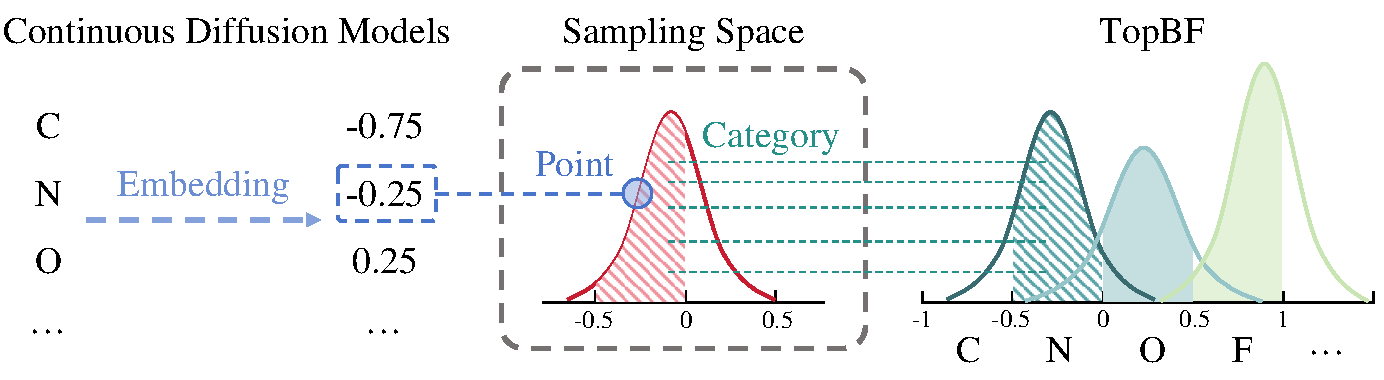
\includegraphics[width=1.\linewidth]{motivation.pdf}
    \caption{Continuous diffusion models are agnostic of the discretization process and only pursue numerical fitting during training, while TopBF directly calculates the probability of each category.}
    \label{fig:motivation}
\end{figure}

Naturally suited for discrete graph structures, discrete diffusion models typically define a forward Markov process that corrupts the graph structure through discrete edits. Conversely, the reverse process learns to restore the graph by framing generation as an iterative classification task \cite{vignac2023digress,xu2024discrete}. 
% DiGress performs a series of discrete and random graph editing operations to diffuse the graph structure, with each editing step following a predefined probability transition rule. During the sampling process, DiGress predicts the original state of each atom and bond in the previous step from the perspective of the classification task. DisCo is a diffusion model based on discrete data and continuous time, using continuous time Markov Chain (CTMC) to define the transition process between states with a rate matrix. 
However, these discrete diffusion models sacrifice the smoother optimization and dynamic generation afforded by continuous representations. Continuous diffusion models have also demonstrated success in this domain \cite{jo2022score,luo2023fast}. They operate on a continuous representation of a graph, involving a forward noising process that incrementally perturbs this representation with continuous noise while training a core network to reverse this corruption.
% EDP-GNN introduces a permutation equivariant graph neural network to model the score function of the graph distribution. GDSS models the joint distribution of the atoms and bonds through a system of stochastic differential equations (SDEs) and applies score matching objectives to estimate the gradient of the joint log-density. 
The primary objective of continuous diffusion models is to predict embedded representations in continuous space and train a neural network to regress those values under injected noise. However, the final output must be discretized by rounding, which is not a benign post-processing step. As shown in Figure~\ref{fig:motivation}, it is evident that throughout the entire training phase, these models remain agnostic regarding the discretization rule. The resulting mismatch between training and sampling can lead to inefficient learning and brittle generation. In particular, point-wise regression errors near category boundaries may be penalized mildly during training but induce catastrophic category flips at inference, which is especially problematic for generation.


% 这一段写得没有前后逻辑
Recently, Bayesian Flow Networks (BFNs) \cite{graves2023bayesian,song2024unified} provide an alternative paradigm for discrete generation by evolving distribution parameters through a continuous-time Bayesian updating process. Instead of directly predicting discrete values, BFNs propagate a parameter state that represents uncertainty and update it via pseudo-observations, yielding a continuous and differentiable learning process for discrete data. 
% However, due to all categories being equidistant within the probability simplex, the model cannot progressively approach objectives in a manner akin to that in continuous space \cite{graves2023bayesian}. As a consequence, this results in a convergence process towards data that appears slower and noisier. 
However, BFNs are not topology-aware for molecular graphs, since they adopt independent Gaussian distributions between variables to retain closed-form Bayesian updates. As a result, BFNs are mainly rewarded for getting each position right in isolation, rather than for capturing how labels should cohere with the overall graph structure.

% 这一段需要好好总结提炼
To address the aforementioned issues, we introduce \textbf{TopBF}, a molecular graph generative BFN that performs generation in continuous distribution-parameter space and uses a CDF-based decoding to compute category probabilities from continuous parameters, thereby aligning the training objective with the same discretization rule used during sampling. Furthermore, we make TopBF topology-aware by introducing a Quasi-Wasserstein transport coupling defined on graph geodesic costs, which compares predicted categorical mass on atoms and bonds with the ground-truth structure. This geometry-respecting discrepancy encourages local, structure-consistent adjustments and discourages topology-inconsistent long-range rearrangements. TopBF also achieves conditional generation via property-error gradient (PEG) guidance.
Notably, TopBF achieves superior performance with the minimum sampling steps, accelerating molecular graph generation in practice.
We summarize our key contributions as follows:

\begin{itemize}
    \item We observe the mismatch defect in continuous diffusion methods and propose TopBF that unifies continuous-parameter training with discrete sampling for MGG.
    \item We inject topology awareness into TopBF training via a Quasi-Wasserstein transport coupling with graph-geodesic ground costs by aligning predicted categorical mass with the molecular structure in a geometry-consistent manner.
    \item TopBF supports training-free and property-conditioned generation via guided sampling while requiring the minimum sampling steps, achieving both effective control and efficient MGG.
\end{itemize}

\section{Related Work}

% \subsubsection{Generative Models for Molecular Graphs.}
Deep generative models for MGG are typically categorized into autoregressive and one-shot models. The former generate graphs incrementally, adding atoms and bonds in an autoregressive manner \cite{you2018graphrnn,jin2018junction,jin2020hierarchical}. 
The latter generate the entire graph at once \cite{simonovsky2018graphvae,luo2021graphdf,martinkus2022spectre}.

% \subsubsection{Diffusion Models for Graph.} 
Diffusion models have been adapted for molecular graph generation \cite{liu2023generative,li2024regressor}. 
% These models learn to reverse a diffusion process that gradually adds noise to the structure and features of a molecular graph. A key issue lies in how to handle the discrete nature of atom and bond labels. 
Some methods define a diffusion process directly on the discrete state space \cite{vignac2023digress,xu2024discrete}, which can be complex to accomplish. Others map discrete attributes to a continuous space and apply standard Gaussian diffusion \cite{huang2022graphgdp,lee2023exploring}.
% however, facing the challenge of accurately converting the final continuous output back to discrete labels without information loss.

% \subsubsection{Bayesian Flow Networks.} 
BFNs have arisen recently to perform generation in continuous parameter distribution \cite{graves2023bayesian,song2024unified,qu2024molcraft}. The process starts with a simple prior distribution and iteratively refines its parameters via Bayesian inference to calculate the posterior from observed samples. 
% A key advantage of BFNs is their ability to create a continuous and differentiable training process for discrete data. The original work achieves this by defining the BFN state as a vector of probabilities on the probability simplex and using multiplicative updates. Our work builds upon the foundational principles of BFNs but proposes a different and simpler mechanism for handling discrete features in the context of molecular graph generation.



\section{Preliminaries}

\subsection{Problem Definition}

A molecular graph $G$ is defined as $(X, A)$, where $X \in \{1, \cdots, K_{X}\}^{D}$ represents a matrix of $D$ atom features derived from $K_X$ classes, and $A \in \{1, \cdots, K_{A}\}^{D \times D}$ denotes an adjacency matrix encapsulating bond features from $K_A$ classes. Here $D$ is the maximum number of atoms in the considered molecules and let $N \leq D$ be the number of valid atoms.

Given a dataset $\mathcal{D} = \{G_i\}_{i=1}^{|\mathcal{D}|}$ sampled from an unknown data distribution $p_{\text{data}}(G)$, the goal of molecular graph generation is to learn a generative model $p_\theta(G)$ that can efficiently sample valid, diverse molecular graphs whose distribution matches $p_{\text{data}}$ in terms of structural and chemical statistics. For the discrete nature of molecular graphs, this task can be seen as a multi-class generative task, where we need to assign specific atomic or chemical bond types at each position subject to chemical validity constraints. In addition, the model may be guided towards desired properties $\mathbf{z}$ to achieve conditional molecular graph generation as a flexible extension.
% In addition, TopBF can be extended to conditional generation, where the model is guided towards molecules with desired properties $\mathbf{y}$, but in this work we focus primarily on the unconditional generative formulation and treat property-guided sampling as a flexible extension.



\subsection{Bayesian Flow Networks}
\label{pre_BFN}
% 还差p_U和p_F，看情况要不要补全 √

Bayesian Flow Networks can be conceptualized as a data transmission protocol between a sender and a receiver. Given data $\mathbf{x}=(x^{(1)}, \cdots, x^{(D)})$, let $\boldsymbol{\theta}=(\theta^{(1)}, \cdots, \theta^{(D)})$ be the parameters of a factorized \emph{input distribution}: $p_I(\mathbf{x}\,|\,\boldsymbol{\theta})=\prod_{d=1}^{D}p_I(x^{(d)}\,|\,\theta^{(d)})$. At each time $t \in [0,1]$, the sender corrupts $\mathbf{x}$ by a Gaussian channel $\alpha$ yielding a \emph{sender distribution}: $p_S(\mathbf{y}\,|\,\mathbf{x};\alpha)=\prod_{d=1}^{D}p_S(y^{(d)}\,|\,x^{(d)};\alpha)$. During the data transmission process, the input parameters $\boldsymbol{\theta}$ are input into a neural network $\Psi$, whose output is then parameterized as an \emph{output distribution}: $p_O(\mathbf{x}\,|\,\boldsymbol{\theta},t)=\prod_{d=1}^{D}p_O(x^{(d)}\,|\,\Psi(\boldsymbol{\theta},t))$. Since the receiver knows the form of the sender distribution but does not know $\mathbf{x}$, it integrates all possible $\mathbf{x}'$ and sender distributions, weighted by the output distribution, and obtains the \emph{receiver distribution}: $p_R(\mathbf{y}\,|\,\boldsymbol{\theta};t, \alpha)=\mathop{\mathbb{E}}\limits_{p_O(\mathbf{x}'|\boldsymbol{\theta};t)}p_S(\mathbf{y}\,|\,\mathbf{x}';\alpha)$. Subsequently, by applying Bayesian inference, \emph{Bayesian update function} $h(\cdot)$ is derived to repeatedly update the parameters: $\boldsymbol{\theta}' = h(\boldsymbol{\theta},\mathbf{y},\alpha)$ along a noise schedule, defined as a continuous-time Bayesian flow $p_F(\boldsymbol{\theta} \mid \mathbf{x};t)$. The \emph{Bayesian update distribution} is then defined by marginalizing out $\mathbf{y}$: $p_U(\boldsymbol{\theta}'\,|\,\boldsymbol{\theta},\mathbf{x};\alpha)=\mathop{\mathbb{E}}\limits_{p_S(\mathbf{y}|\mathbf{x};\alpha)}\delta(\boldsymbol{\theta}'-h(\boldsymbol{\theta},\mathbf{y},\alpha))$, where $\delta(\cdot)$ is the Dirac delta distribution. Now define the \emph{accuracy schedule} $\beta(t)$ as $\beta(t)=\int_{t'=0}^{t}\alpha(t')dt'$, and the \emph{Bayesian flow distribution} is the marginal distribution over input parameters at time $t$: $p_F(\boldsymbol{\theta}\,|\,\mathbf{x};t)=p_U(\boldsymbol{\theta}\,|\,\boldsymbol{\theta}_0;\mathbf{x};\beta(t))$.

\subsection{Optimal Transport and Quasi-Wasserstein Coupling on Graphs}
\label{sec:prelim_ot}

Optimal transport (OT) provides a geometry-aware way to compare two distributions by measuring the minimum cost required to move probability mass from one to the other \cite{gabriel2019computational}. Consider a molecular graph $G=(X,A)$ with $N$ atoms, and let $C\in\mathbb{R}_+^{N\times N}$ be the geodesic ground-cost matrix induced by the shortest-path metric on $G$, i.e., $C_{ij}=\mathrm{dist}_{G}(i,j)$. Given two probability distributions $\mathbf{a},\mathbf{b}\in\Delta^{N-1}$ over atom indices, the entropically regularized OT cost is
$
\mathcal{W}_{\varepsilon}(\mathbf{a},\mathbf{b};C)
=
\min_{P\in\Pi(\mathbf{a},\mathbf{b})}
\langle P, C\rangle
+
\varepsilon\sum_{i,j} P_{ij}\big(\log P_{ij}-1\big)$, where $
\Pi(\mathbf{a},\mathbf{b})=\{P\ge 0\mid P\mathbf{1}=\mathbf{a},~P^\top\mathbf{1}=\mathbf{b}\}$. In practice, we solve the entropy-regularized OT and obtain the coupling $P$ via Sinkhorn iterations \cite{cuturi2013sinkhorn}.

Quasi-Wasserstein (QW) extends this idea from comparing single scalar signals on atoms to comparing multi-class label fields on graphs. Specifically, for a categorical field with $K$ classes, we view category probability map $P(\cdot,k)\in[0,1]^N$ as a mass distribution over atom indices for each class $k$, and compare prediction $P(\cdot,k)$ and target $Q(\cdot,k)$ by transporting mass within each class under the same geodesic cost $C$. The QW discrepancy then aggregates these per-class transport costs: 
$
\mathcal{D}_{\mathrm{QW}}(P,Q;C)
=
\frac{1}{K}\sum_{k=1}^{K}
\mathcal{W}_{\varepsilon}\!\big(\mathbf{a}_k,\mathbf{b}_k;C\big),
\mathbf{a}_k=\mathrm{Norm}\!\big(P(\cdot,k)\big),
\mathbf{b}_k=\mathrm{Norm}\!\big(Q(\cdot,k)\big),
$
where $\mathrm{Norm}(\cdot)$ denotes normalization to the simplex on valid atoms. In contrast to position-wise divergences, $\mathcal{D}_{\mathrm{QW}}$ penalizes errors according to how far probability mass moves along the graph, encouraging local and topology-consistent corrections while discouraging long-range and structure-inconsistent reallocations.



\begin{figure*}
    \centering
    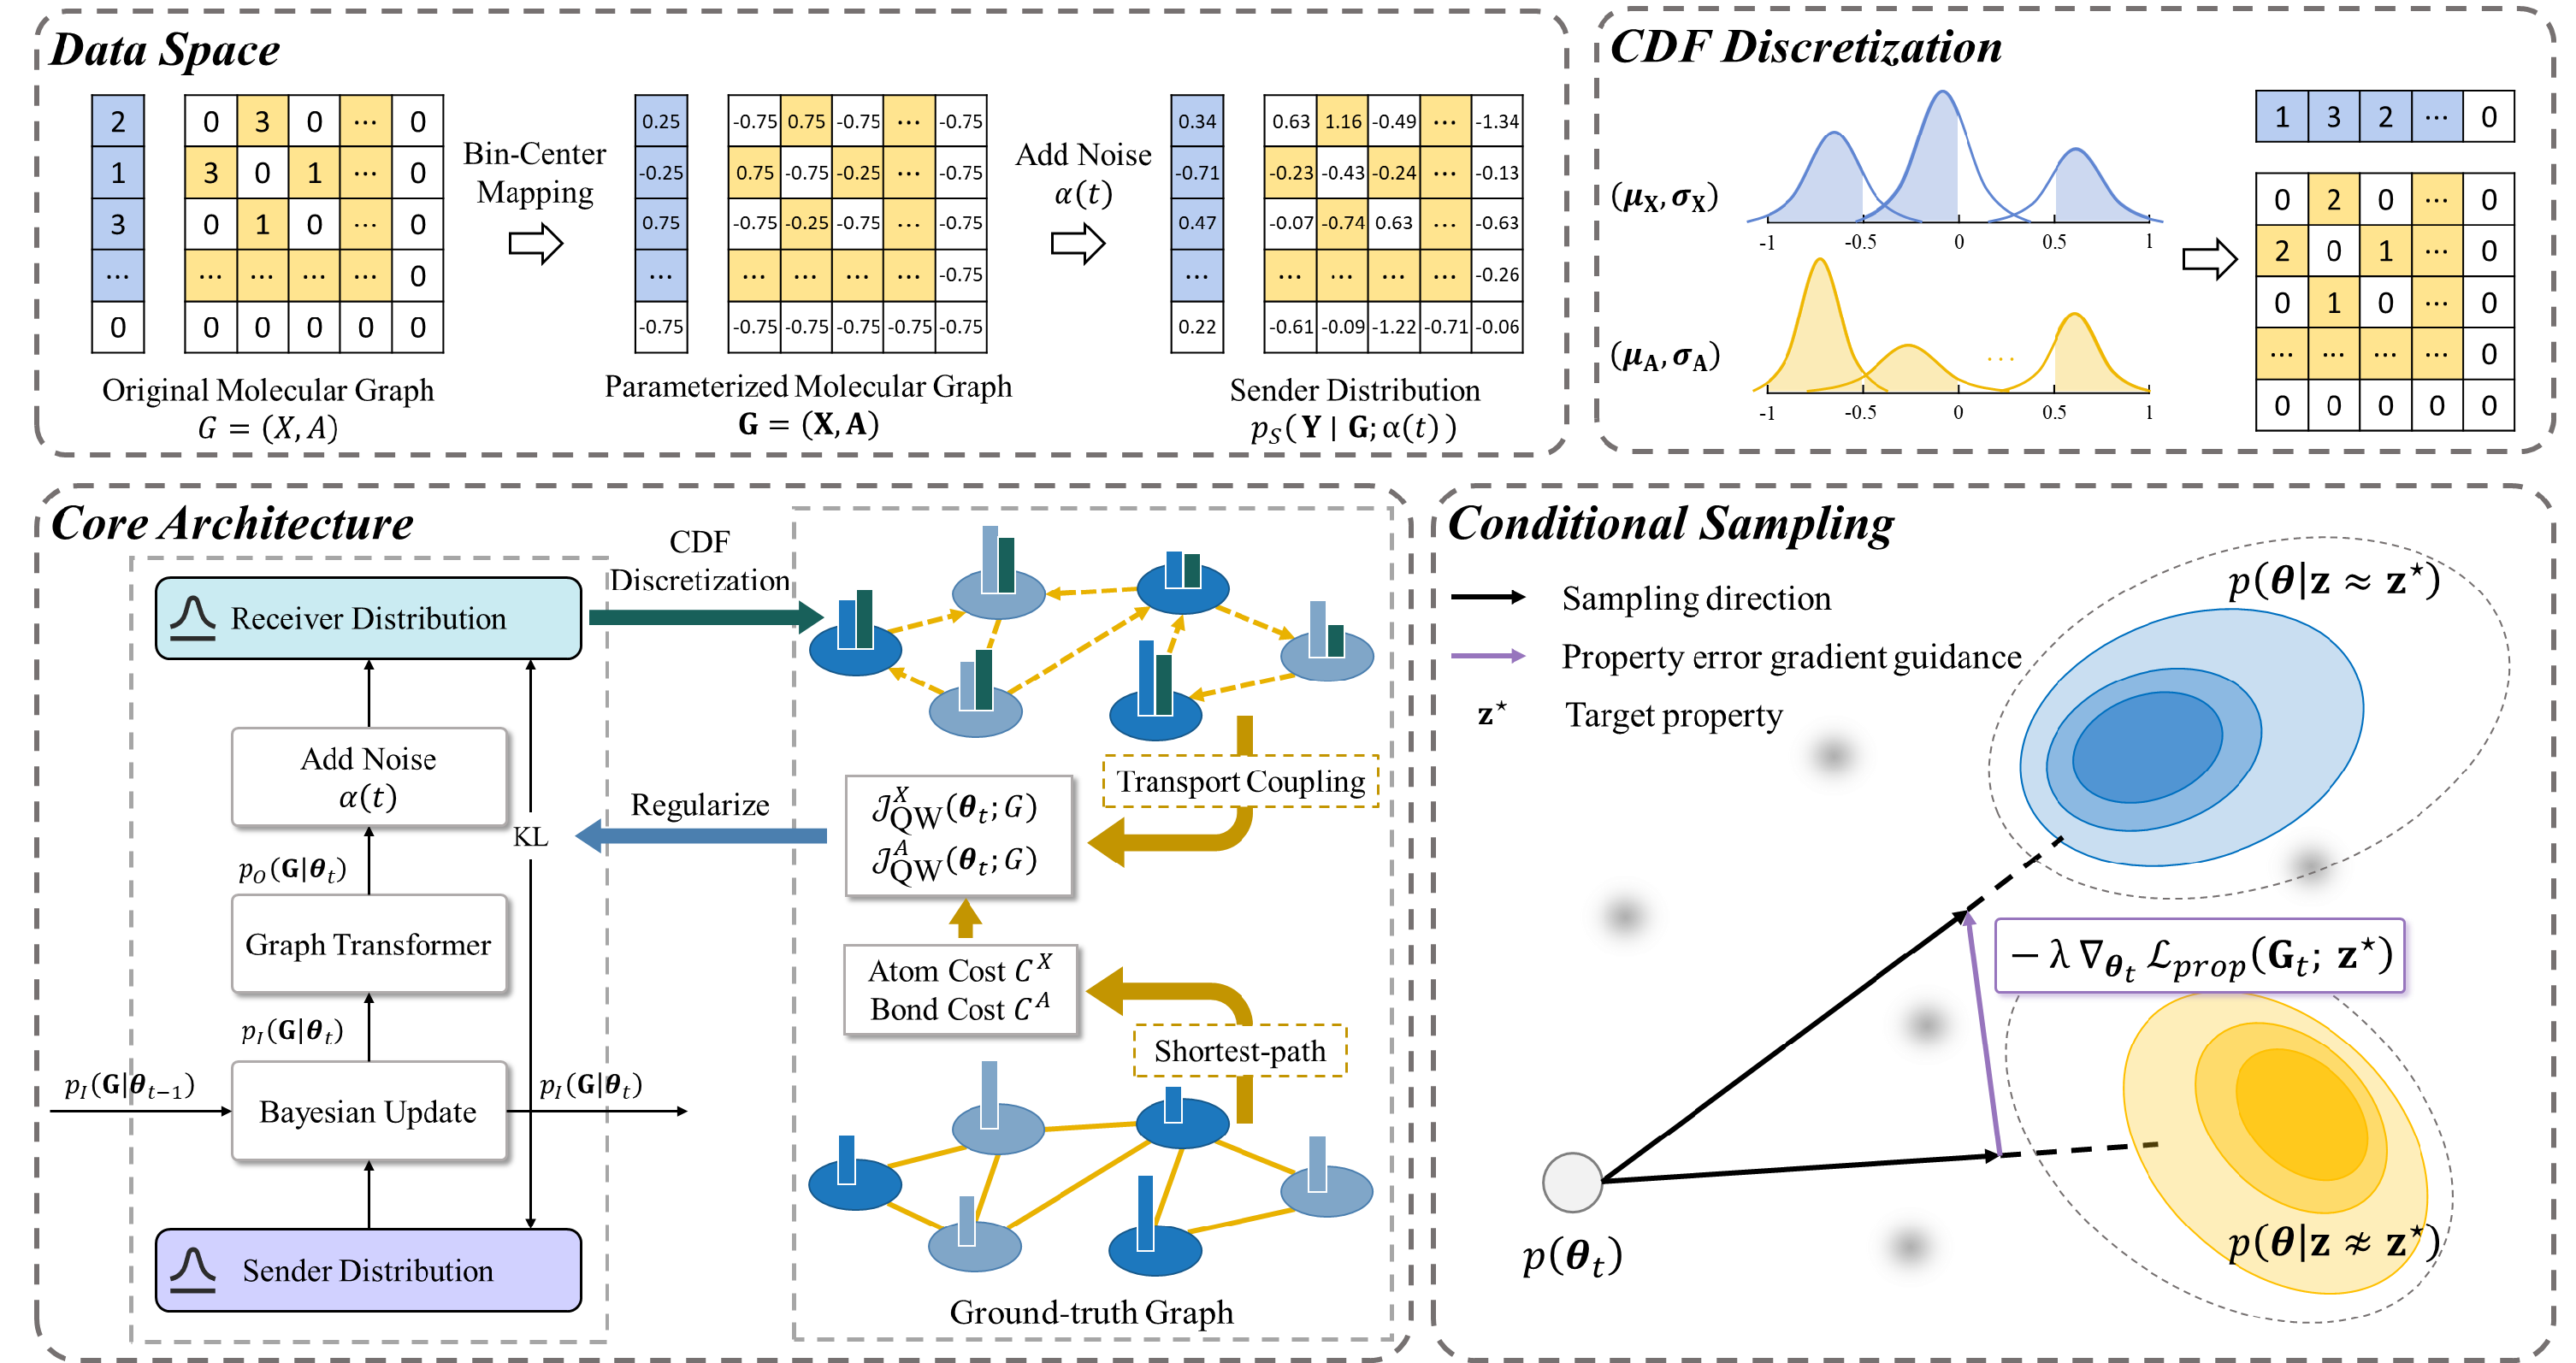
\includegraphics[width=1.\linewidth]{model.pdf}
    \caption{Overall framework of TopBF. \textbf{Data Space}: The procedure of parameterizing and adding noise to the molecular graph for the sender distribution. \textbf{CDF Discretization}: Obtain atom and bond categories from the output of $\Psi$ through CDF. \textbf{Core Architecture}: The structure of a BFN module at time $t$. And a QW transport coupling regularizes the training procedure. \textbf{Conditional Sampling}: PEG guidance for conditional generation.}
    \label{fig:model}
\end{figure*}

\section{Materials and Methods} % 计算损失的时候，有一部经过推理是可以不用计算加噪后的原数据的，确认一下有没有写
% 这一节要提到和扩散模型的本质区别！！！！！！！！！！！

In this section, we describe how our MGG framework, \underline{\textbf{T}}ransp\underline{\textbf{o}}rt-Cou\underline{\textbf{p}}led \underline{\textbf{B}}ayesian \underline{\textbf{F}}lows (TopBF), generates molecular graphs via Bayesian flows over continuous distribution parameters, as illustrated in Figure~\ref{fig:model}. Pseudocodes for training and sampling are provided in Appendix 8. % "into a flow"的表述准确吗？？？？？

\subsection{Datasets and Metrics} 
% We choose QM9 \cite{ramakrishnan2014quantum} and ZINC250k \cite{irwin2012zinc} for molecular graph generation.

We validate our approach on the QM9 \cite{ramakrishnan2014quantum} and ZINC250k \cite{irwin2012zinc} benchmarks, following the previous experimental setup \cite{jo2022score}. QM9 contains approximately 133,885 molecules with up to 9 heavy atoms of 4 types, while ZINC250k comprises roughly 249,455 molecules with up to 38 heavy atoms of 9 types, both covering three standard bond types. Adhering to the standard pipeline \cite{luo2021graphdf,jo2022score}, molecules undergo kekulization via RDKit, with explicit hydrogens excluded to focus on the heavy-atom graph representation.

We evaluate the experiments following previous evaluation setting \cite{jo2022score}: Validity without correction and uniqueness on 10,000 generated molecules. Fréchet ChemNet Distance (FCD) \cite{preuer2018frechet} measures the distance between training and generated sets using the activations from the penultimate layer of the ChemNet. Additionally, Neighborhood Subgraph Pairwise Distance Kernel (NSPDK) maximum mean discrepancy (MMD) \cite{costa2010fast} evaluates the MMD between the generated molecules and test molecules which takes into account both the atom and bond features for evaluation.



% \subsection{Continuous Parameterization of Molecular Graphs}
\subsection{Parameterization of Molecular Graphs}
% 前后文的class, interval, bin，最好统一换成class


% 解释为什么映射是必要的 √
Since directly manipulating discrete data often leads to more complex operations to guarantee differentiability, a foundational step of our method involves mapping the discrete atom and bond features into continuous spaces. For a feature class $k \in \{1, \cdots, K\}$, we define a deterministic mapping to a continuous value $x_k \in [-1, 1]$:
% \begin{equation}
%     \begin{aligned}
%         \left\{
%     \begin{aligned}
%         & k_c = \frac{2k-1}{K} - 1, \\
%         & k_l = k_c - \frac{1}{K}, \\
%         & k_r = k_c + \frac{1}{K}, \\
%     \end{aligned}
%     \right.
%     \end{aligned}
% \label{eq:class-mapping}
% \end{equation}
\begin{equation}
    k_c = \frac{2k-1}{K} - 1, \quad k_l = k_c - \frac{1}{K},\quad k_r = k_c + \frac{1}{K},
\label{eq:class-mapping}
\end{equation}
where $k_l$, $k_c$ and $k_r$ represent the respective vectors for left boundaries, centers and right boundaries of the classes. Importantly, we assign the continuous value $x_k \coloneqq k_c$ to the $k$-th class. This mapping transforms the ground-truth graph $G$ into continuous representation $\mathbf{G}=(\mathbf{X}, \mathbf{A})$. This continuous representation serves as the target signal for generative flow.

\subsection{Bayesian Flow Over Distribution Parameters}


\subsubsection{Input distribution in parameter space.} % From continuous
% 注意mu是否加粗，BFN中出现了两种形式。
% -> 应该要加粗，加粗的表示向量，反之则是单值
Instead of modeling $G$ directly as diffusion models, TopBF operate on parameters of a simple input distribution over continuous $\mathbf{G}$. For each of atoms and bonds we maintain a Gaussian input distribution:
\begin{align}
    p_I(\mathbf{X} \mid \boldsymbol{\theta}_\mathbf{X}) &= \mathcal{N}(\mathbf{X} \mid \boldsymbol{\mu}_\mathbf{X}, \rho_\mathbf{X}^{-1}\boldsymbol{I}), \\
    p_I(\mathbf{A} \mid \boldsymbol{\theta}_\mathbf{A}) &= \mathcal{N}(\mathbf{A} \mid \boldsymbol{\mu}_\mathbf{A}, \rho_\mathbf{A}^{-1}\boldsymbol{I}),
\end{align}
where $\boldsymbol{\theta} \overset{def}{=} (\boldsymbol{\mu}, \rho)$ consists of a mean vector $\mu \in \mathbb{R}^D$ and a scalar precision $\rho > 0$, and $\boldsymbol{I}$ is the $D \times D$ identity matrix. The process initiates with a standard normal prior $p_I(\cdot \mid \boldsymbol{\theta}_0) = \mathcal{N}(\cdot \mid \boldsymbol{0}, \boldsymbol{I})$ at time $t=0$. 
For brevity, we will use the integrated form in our formulas: $p_I(\mathbf{G} \mid \boldsymbol{\theta}) = \mathcal{N}(\mathbf{G} \mid \boldsymbol{\mu}, \rho^{-1}\boldsymbol{I})$, except in special circumstances. 

\subsubsection{Sender distribution: adding noise to the data.}
Given continuous $\mathbf{G}=(\mathbf{X}, \mathbf{A})$, the sender distribution plays a role forwarding noising data. For each time-dependent accuracy parameter $\alpha(t)$, the sender draws a noisy message:
\begin{equation}
    p_S(\mathbf{Y} \mid \mathbf{G}; \alpha(t)) = \mathcal{N}(\mathbf{Y} \mid \mathbf{G}, \alpha(t)^{-1}\boldsymbol{I}),
\label{eq:sender}
\end{equation}
where $\mathbf{Y} = (\mathrm{Y}^{(1)}, \cdots, \mathrm{Y}^{(D)})$ is a noisy observation of the true graph, whose noise level increases when $\alpha(t)$ is small.

\subsubsection{Bayesian update and Bayesian flow distribution.}
BFNs define a Bayesian update that combines the current input distribution $p_I(\mathbf{G} \mid \boldsymbol{\theta})$ with a noisy observation $\mathbf{Y}$ from the sender, yielding a posterior over $\mathbf{G}$ that can again be written as a Gaussian in closed form. Since both $p_I$ and $p_S$ are Gaussians with diagonal covariances, the Bayesian update for each of atoms and bonds reduces to \cite{murphy2007conjugate}:
\begin{equation} % 这个公式查一下正确性；加粗符号
\label{eq:bayes-update}
\begin{aligned}
        \left\{
\begin{aligned}
    \rho_i &= \rho_{i-1} + \alpha, \\
    \boldsymbol{\mu}_i  &= \frac{\rho_{i-1} \boldsymbol{\mu}_{i-1} + \alpha \mathbf{Y}}{\rho_{i-1} + \alpha}.
\end{aligned}
\right.
\end{aligned}
\end{equation}
Repeating this update along a schedule of accuracies induces a stochastic trajectory $\{\boldsymbol{\theta}_t\}_{t \in [0,1]}$ in parameter space that converges towards the true graph $\mathbf{G}$ as $t \to 1$.

Rather than explicitly simulating all intermediate steps, there exists a \emph{Bayesian flow distribution} $p_F(\boldsymbol{\theta}\,|\,\mathbf{G}; t)$ describing the distribution of input parameters at time $t$ after aggregating all past Bayesian updates, detailed in Sec.~\ref{pre_BFN}.
% In practice, we can sample $\boldsymbol{\theta}_t \sim p_F(\boldsymbol{\theta} \mid \mathbf{G}; t)$ for random $t \sim \mathcal{U}(0,1)$ and train the core network using Monte Carlo estimates of the flow loss.

Conceptually, the dynamics are defined on \emph{distribution parameters} $(\boldsymbol{\mu}, \rho)$ rather than on data itself. This is the key distinction of TopBF from standard diffusion models.



\subsection{Output and Receiver Distributions for Molecular Graphs}

The core neural network in TopBF takes as input the current parameter state $\boldsymbol{\theta}_t$ and time $t$, and outputs a prediction of the Gaussian noise used to generate the input mean. We denote the network by:
\begin{equation}
    \boldsymbol{\epsilon} = \Psi(\boldsymbol{\theta}_t, \mathbf{c}, t),
\end{equation}
where $\mathbf{c}$ represents any optional conditioning. The output $\boldsymbol{\epsilon}$ is split into two $D$-dimensional vectors $(\boldsymbol{\mu}_\epsilon, \ln \boldsymbol{\sigma}_\epsilon)$, which are then transformed into the mean and standard deviation $(\hat{\boldsymbol{\mu}}_\mathbf{G}, \hat{\boldsymbol{\sigma}}_\mathbf{G})$ of a Gaussian over the continuous data (formal derivation of the transformation in Appendix 1):
\begin{equation}
    \begin{aligned}
        & \hat{\boldsymbol{\mu}}_\mathbf{G} = \left\{
    \begin{aligned}
        & \, \boldsymbol{0} & \text{if $t<t_{\text{min}}$},\\
        & \frac{\boldsymbol{\mu}}{\gamma(t)} - \sqrt{\frac{1-\gamma(t)}{\gamma(t)}}\boldsymbol{\mu}_\epsilon & \text{otherwise,}
    \end{aligned}
    \right. \\
    & \hat{\boldsymbol{\sigma}}_\mathbf{G} = \left\{
    \begin{aligned}
        & \, \boldsymbol{1} & \text{if $t<t_{\text{min}}$},\\
        & \sqrt{\frac{1-\gamma(t)}{\gamma(t)}}\text{exp}(\ln\boldsymbol{\sigma}_\epsilon) & \text{otherwise,}
    \end{aligned}
    \right.
    \end{aligned}
\label{eq:mu-sigma-x}
\end{equation}
where $\gamma(t) = \beta(t)/(1 + \beta(t))$ is determined by the accuracy schedule $\beta(t)$ of BFNs, and $t_{\min}$ is a small positive constant to avoid numerical issues at $t=0$.


% \begin{figure*} % 考虑放到附录，这样可以多放一些分子图
%     \centering
%     \includegraphics[width=0.95\linewidth]{samples.pdf}
%     \caption{Samples generated by TopBF on ZINC250k and QM9 datasets.}
%     \label{fig:samples}
% \end{figure*}


\subsubsection{Truncated Gaussian CDF and per-class probabilities.}
While Eq.~\eqref{eq:mu-sigma-x} defines a continuous Gaussian distribution over $\mathbf{G}$, our ultimate goal is to make discrete predictions over $K$ classes. To bridge this gap, TopBF uses a truncated Gaussian cumulative distribution function (CDF) to compute the probability mass assigned to each discretization class.

For each dimension $d \in \{1,\cdots,D\}$, we define the Gaussian CDF:
\begin{equation}
    F(x \mid \mu_x^{(d)}, \sigma_x^{(d)}) = \frac{1}{2}\Bigg[ 1 + \text{erf} \left( \frac{x-\mu_x^{(d)}}{\sqrt{2}\sigma_x^{(d)}} \right) \Bigg],
\label{eq:gauss-cdf}
\end{equation}
where $\text{erf}(\cdot)$ is the error function defined as $\text{erf}(u)=\frac{2}{\sqrt{\pi}}\int_{0}^{u}e^{-t^2}dt$. Here truncate the support to the interval $[-1, 1]$ to align with the embedding range:
\begin{equation}
    \begin{aligned}
        & \mathcal{F}(x \,|\, \mu_x^{(d)}, \sigma_x^{(d)}) = \left\{
        \begin{aligned}
            & \, 0 & \text{if $ x \leq -1$ },\\
            & \, 1 & \text{if $ x \geq 1 $}, \\
            & F(x \,|\, \mu_x^{(d)}, \sigma_x^{(d)}) & \text{otherwise, }
        \end{aligned}
        \right.
    \end{aligned}
\end{equation}
Using the class boundaries $(k_l, k_r)$ from Eq.~\eqref{eq:class-mapping}, the probability of assigning dimension $d$ to category $k \in \{1, \cdots K\}^D$ is determined by the integral of the truncated Gaussian over the corresponding class:
\begin{equation}
    p_O^{(d)}(k \mid \boldsymbol{\theta}_t) = \mathcal{F}(k_r \mid \mu_x^{(d)}, \sigma_x^{(d)}) - \mathcal{F}(k_l \mid \mu_x^{(d)}, \sigma_x^{(d)}).
\label{eq:po-discrete}
\end{equation}
To achieve closed-form \emph{Bayesian update}, the output distribution over the $\mathbf{G}$ is independent across dimensions:
\begin{equation}
    p_O(\mathbf{G} \mid \boldsymbol{\theta}_t) = \prod_{d=1}^{D}p_O^{(d)}\Big( k(\mathrm{G}^{(d)}) \mid \boldsymbol{\theta}_t \Big),
\label{eq:po-factorised}
\end{equation}
where $k(x^{(d)})$ denotes the index of the class occupied by $x^{(d)}$. Similarly, we define the expected class-center representation under the current output distribution as:
\begin{equation}
    \begin{aligned}
        & \mathbb{E}[P(\boldsymbol{\theta}, t)] = \hat{\mathbf{k}}(\boldsymbol{\theta}, t) \\
        \overset{def}{=} & \left( \sum_{k=1}^{K}p^{(1)}(k \,|\, \boldsymbol{\theta}, t) k_{c}, \cdots, \sum_{k=1}^{K}p^{(D)}(k \,|\, \boldsymbol{\theta}, t) k_{c} \right).
    \end{aligned}
\end{equation}




\subsubsection{Receiver distribution as a mixture of Gaussians.}
The receiver distribution $p_R$ inverts the sender process in parameter space by describing the distribution over noisy messages $\mathbf{Y}$ implied by the current parameter state $\boldsymbol{\theta}_t$. Consequently, substituting Eqs.~\eqref{eq:sender} and~\eqref{eq:po-discrete} into the BFN formulation yields a mixture of Gaussians:
\begin{equation}
    \begin{aligned}
        & p_R(\mathbf{Y} \mid \boldsymbol{\theta}; t, \alpha(t)) = \mathop{\mathbb{E}}\limits_{p_O(\mathbf{G} \mid \boldsymbol{\theta}_t)} p_S(\mathbf{Y} \mid \mathbf{G}; \alpha(t)), \\
        & = \prod_{d=1}^D \sum_{k=1}^{K}p_O^{(d)}(k \mid \boldsymbol{\theta}_t) \mathcal{N}(\mathrm{Y}^{(d)} \mid k_c, \alpha(t)^{-1}).
    \end{aligned}
\label{eq:receiver-discrete}
\end{equation}
The receiver plays the role of the \emph{reverse} channel in the flow. During training, we encourage the receiver distribution to match the sender distribution applied to $\mathbf{G}$, while during sampling it serves to generate pseudo-observations that drive the Bayesian updates in Eq.~\eqref{eq:bayes-update}. Notably, TopBF applies the above construction independently to atoms and bonds by using $K = K_X$ and $K = K_A$, respectively.


\subsection{Topology-aware Optimal Transport Matching}
\label{sec:topo_ot}

Although the position-wise factorization in Eq.~\eqref{eq:po-factorised} enables closed-form Bayesian updates, it also yields largely local and index-wise supervision that does not explicitly encode graph topology. However, categorical errors are not equally severe, since swapping mass within a local neighborhood is structurally less disruptive than relocating it across distant substructures \cite{frogner2015learning,cheng2024quasi}. To bridge this gap, we introduce an OT coupling that regularizes predictions under molecule's intrinsic geometry.

\subsubsection{Graph-induced Ground Cost.}
We define the atom-level ground cost by the shortest-path metric: 
\begin{equation}
    C^{X}_{ij} \;=\; \mathrm{dist}_{G}(i,j),\qquad i,j\in\{1,\cdots,N\}.
\label{eq:cost_X}
\end{equation}
For bonds, we define an bond-level cost $C^{A}$ using an endpoint-based proxy consistent with our implementation, e.g., for two undirected bonds $e=(i,j)$ and $e'=(u,v)$,
\begin{equation}
\begin{aligned}
C^{A}_{e,e'} = \min \big\{ & \mathrm{dist}_{G}(i,u), \mathrm{dist}_{G}(i,v), \\
& \mathrm{dist}_{G}(j,u), \mathrm{dist}_{G}(j,v) \big\}.
\label{eq:cost_A}
\end{aligned}
\end{equation}
% This cost quantifies the topological effort required to reconcile probability mass across different indices, discouraging rearrangements that violate the molecular structure.
\begin{theorem}[Endpoint proxy matches line-graph geodesics]
\label{thm:line_graph}
Let $\mathcal{L}(G)$ be the line graph of $G$ whose vertices correspond to bonds and edges connect bonds that share an endpoint. For any two distinct undirected bonds $e,e'$,
\[
\mathrm{dist}_{\mathcal{L}(G)}(e,e') \;=\; 1 + C^{A}_{e,e'} .
\]
\end{theorem}
Thus, $C^{A}$ differs from the exact line-graph geodesic only by an additive constant and induces the same optimal OT coupling (proof in Appendix 3).

\subsubsection{Optimal Transport over Categorical Mass.}
We make topology awareness a first-class objective by minimizing the transport work needed to align predicted categorical mass with the ground truth \cite{peyre2016gromov}.
At time $t$, a sample $\boldsymbol{\theta}_t\sim p_F(\boldsymbol{\theta} \,|\, \mathbf{G};t)$ yields categorical probabilities from Eq.~\eqref{eq:po-factorised}, with targets $Q_X,Q_A$. We form class-wise mass fields by normalizing $P_X(\cdot,k)$ and $P_A(\cdot,k)$ on valid indices and only aggregate over classes that appear in the true graph $G$: $\mathcal{K}_X^{+}(G)=\{k \mid \exists\, i \ \text{s.t.}\ X_i=k\}$ and $\mathcal{K}_A^{+}(G)=\{k \mid \exists\, e \ \text{s.t.}\ A_e=k\}$. Thus we define the QW transport costs

\begin{align}
\mathcal{J}^{X}_{\mathrm{QW}}(\boldsymbol{\theta}_t;G)
&=
\frac{1}{|\mathcal{K}_X^{+}(G)|}
\sum_{k\in\mathcal{K}_X^{+}(G)}
\!\mathcal{W}_{\varepsilon}\!\big(\mathbf{a}_k^X,\mathbf{b}_k^X;C^{X}\big),
\label{eq:qw_X}
\\
\mathcal{J}^{A}_{\mathrm{QW}}(\boldsymbol{\theta}_t;G)
&=
\frac{1}{|\mathcal{K}_A^{+}(G)|}
\sum_{k\in\mathcal{K}_A^{+}(G)}
\!\mathcal{W}_{\varepsilon}\!\big(\mathbf{a}_k^A,\mathbf{b}_k^A;C^{A}\big),
\label{eq:qw_A}
\end{align}
where $\mathcal{W}_{\varepsilon}$ is the entropic OT cost in Sec.~\ref{sec:prelim_ot}; for bonds we exclude the  invalid bond class from $\mathcal{K}_A^{+}(G)$ to avoid trivial domination. The overall training objective then minimizes the expected transport work induced by the receiver predictions, 
% \begin{equation}
% \min\ \mathcal{L}_{G}
% +
% \lambda_{\mathrm{OT}}\,
% \mathbb{E}_{t\sim\mathcal{U}(0,1),\,\boldsymbol{\theta}_t\sim p_F(\boldsymbol{\theta}\mid G;t)}
% \Big[
% \mathcal{J}^{X}_{\mathrm{QW}}(\boldsymbol{\theta}_t,t;G)
% +
% \mathcal{J}^{A}_{\mathrm{QW}}(\boldsymbol{\theta}_t,t;G)
% \Big],
% \label{eq:total_topo_objective}
% \end{equation}
% which encourages topology-consistent predictions by construction.

\begin{theorem}[Hard-label limit of class-wise transport]
\label{thm:em}
Fix a class $k$ and suppose $\mathbf{a}_k=\frac{1}{r}\sum_{\ell=1}^{r}\mathbf{e}_{i_\ell}$ and $\mathbf{b}_k=\frac{1}{r}\sum_{\ell=1}^{r}\mathbf{e}_{j_\ell}$ are uniform sums of $r$ Diracs. Then
\[
\mathcal{W}_{0}(\mathbf{a}_k,\mathbf{b}_k;C)
=
\frac{1}{r}\min_{\pi\in\mathfrak{S}_r}\sum_{\ell=1}^{r} C_{i_\ell,j_{\pi(\ell)}}.
\]
\end{theorem}
Proof is in Appendix 4.2.


\begin{table*}
  \centering
  \caption{Performance comparison on QM9 and ZINC250k datasets. The best results are highlighted in \textbf{bold} and the second best are \underline{underlined}. Null values (-) in criteria indicate that statistics are unavailable from the original paper.}
  \renewcommand \arraystretch{1.}
  \begin{tabular*}{\textwidth}{@{\extracolsep{\fill}}lccccccccc@{\extracolsep{\fill}}}
    \hline

    \multirow{2}{*}{Method} & \multicolumn{4}{c}{QM9$_{\,\, (|N|\leq\text{9})}$} & \multicolumn{4}{c}{ZINC250k$_{\,\, (|N|\leq\text{38})}$} & \multirow{2}{*}{\makecell[c]{Sampling \\ Steps}} \\
    \cmidrule(lr){2-5} \cmidrule(lr){6-9}
     & $\text{Valid(\%)}\uparrow$ & Unique$\uparrow$ & FCD$\downarrow$ & NSPDK$\downarrow$ & $\text{Valid(\%)}\uparrow$ & Unique$\uparrow$ & FCD$\downarrow$ & NSPDK$\downarrow$ \\
    \hline
    % MoFlow & 91.36 & 98.65 & 4.467 & 0.0169 & 63.76 & 99.99 & 20.875 & 0.0468 & - \\
    EDP-GNN & 47.52 & \underline{99.25} & 2.680 & 0.0046 & 82.97 & 99.79 & 16.737 & 0.0485 & 1000 \\
    % GraphEBM & 8.22 & 97.90 & 6.143 & 0.0287 & 5.29 & 98.79 & 35.467 & 0.2089 & - \\
    GDSS & 95.72 & 98.46 & 2.900 & 0.0033 & 97.01 & 99.64 & 14.656 & 0.0195 & 1000 \\
    DiGress & 98.19 & 96.20 & \underline{0.095} & 0.0003 & 94.99 & 99.97 & 3.482 & 0.0021 & 500 \\
    % GSDM & \textbf{99.90} & - & 2.614 & 0.0034 & 92.57 & - & 12.435 & 0.0168 & 1000 \\
    % Flow Matching & 94.10 & 98.20 & 5.155 & - & 94.01 & 96.68 & 18.764 & - \\
    % Dirichlet FM & 99.10 & 98.15 & 0.888 & 0.0041 & 97.52 & 99.20 & 14.222 & 0.0328 & 400 \\
    % CatFlow & 99.81 & 99.95 & 0.441 & 0.0029 & 99.21 & \textbf{100.00} & 13.211 & 0.0207 & - \\
    LGD-large & 99.13 & 96.82 & 0.104 & \underline{0.0002} & - & - & - & - & 1000 \\
    GruM & \underline{99.69} & 96.90 & 0.108 & \underline{0.0002} & 98.65 & 99.97 & 2.257 & 0.0015 & 1000 \\
    DeFoG & 99.30 & 96.30 & 0.120 & - & 99.22 & \underline{99.99} & \underline{1.425} & \textbf{0.0008} & 1000 \\
    SID & 99.67 & 95.66 & 0.504 & \textbf{0.0001} & \textbf{99.50} & 99.84 & 2.010 & 0.0021 & 500 \\
    \hline
    % $\text{TopBF}_\text{w/o}$ & 99.54 & \underline{99.03} & 0.143 & 0.0002 & 97.66 & \textbf{100.00} & \textbf{4.028} & \textbf{0.0042} & \textbf{200} \\
    $\text{TopBF}$ & \textbf{99.74} & \textbf{99.27} & \textbf{0.093} & \underline{0.0002} & \underline{99.37} & \textbf{100.00} & \textbf{1.392} & \textbf{0.0008} & \textbf{200} \\
    
    \hline
  \end{tabular*}
  \label{tab:1}
\end{table*}


\subsection{Training Objective}
\label{BFN Loss}

The BFN loss can be interpreted either as the number of nats required to transmit the data through the Bayesian flow, or equivalently as the negative variational lower bound over message sequences. Concretely, we sample $t\sim\mathcal{U}(0,1)$ and $\boldsymbol{\theta}_t\sim p_F(\boldsymbol{\theta}\mid \mathbf{G};t)$, and minimize the expected divergence between the sender distribution applied to the ground-truth discretized graph and the receiver distribution implied by $\boldsymbol{\theta}_t$: 
\begin{equation}
\!\mathcal{L}_{\mathbf{G}}
\!=\!
\mathop{\mathbb{E}}\limits_{t,\boldsymbol{\theta}_t}
\Big[
{\mathrm{KL}}\!\Big(
p_S(\mathbf{Y} | \mathbf{G};\alpha(t))
\big\Vert
p_R(\mathbf{Y} | \boldsymbol{\theta}_t; t,\alpha(t))
\Big)
\Big].
\label{eq:bfn_cont_time_kl}
\end{equation}

In TopBF, $p_S$ and $p_R$ are Gaussians with diagonal covariance and we adopt the accuracy schedule $\alpha(t)=\sigma_1^{-2t}$. For a single continuous feature, it makes the KL divergence proportional to a squared error between the true value and the receiver mean. For discretized atom and bond features, we represent each category by $k_c$ in the one-dimensional continuous space and use the expectation of these centers under $p_O$. Here it yields the continuous-time losses for atoms and bonds  (Appendix 2 for a detailed derivation):
\begin{equation}
\label{eq:atom-loss}
    \!\!\mathcal{L}_{\mathbf{X}}
    = - \ln \sigma_{1} \,
    \mathop{\mathbb{E}}\limits_{t \sim \mathcal{U}(0,1),\, p_F(\boldsymbol{\theta} \mid \mathbf{X}; t)}
    \!\!\left[
        \frac{\big\| \mathbf{X} - \hat{\mathbf{k}}_{\mathbf{X}} (\boldsymbol{\theta}, t) \big\|_2^2}
             {\sigma_{1}^{2t}}
    \right],
\end{equation}
where $\sigma_{1}$ is the target standard deviation of the input distribution at $t=1$. An analogous loss $\mathcal{L}_A$ is defined for bond features and the base objective is $ \mathcal{L}_{\mathbf{G}} = \mathcal{L}_{\mathbf{X}} + \mathcal{L}_{\mathbf{A}}$.

To inject explicit topology awareness into training, we further minimize the expected Quasi-Wasserstein transport work defined in Sec.~\ref{sec:topo_ot}: 
\begin{equation}
% \lambda_{\mathrm{OT}}\,
\mathop{\mathbb{E}}\limits_{t\sim\mathcal{U}(0,1),\,\boldsymbol{\theta}_t\sim p_F(\boldsymbol{\theta}\mid \mathbf{G};t)}
\Big[
\mathcal{J}^{X}_{\mathrm{QW}}(\boldsymbol{\theta}_t; \mathbf{G})
+
\mathcal{J}^{A}_{\mathrm{QW}}(\boldsymbol{\theta}_t; \mathbf{G})
\Big].
\label{eq:total_topo_objective}
\end{equation}
This joint objective preserves the original Bayesian flow formulation while encouraging predictions that align with the ground-truth graph through low-cost geodesic transport.


\begin{table}
  \centering
  \caption{Comparison on MAE between unconditional generation and PEG guidance generation.}
  \renewcommand \arraystretch{1.}
  \begin{tabular*}{\columnwidth}{@{\extracolsep{\fill}}ccccc@{\extracolsep{\fill}}}
    \hline

    \multicolumn{2}{c}{Target} & $\mu\downarrow$ & HOMO$\downarrow$ & $\mu$ \& HOMO$\downarrow$ \\
    \hline
    \multicolumn{2}{c}{Unconditional} & $\text{1.69}_{\pm\text{0.05}}$ & $\text{0.96}_{\pm\text{0.01}}$ & $\text{1.73}_{\pm\text{0.02}}$ \\
    \hline
    \multirow{3}{*}{+PEG} & $\lambda=0.5$ & $\text{0.92}_{\pm\text{0.04}}$ & $\text{0.71}_{\pm\text{0.02}}$ & $\text{0.93}_{\pm\text{0.03}}$ \\
     & $\lambda=1.0$ & $\textbf{0.63}_{\pm\text{0.04}}$ & $\textbf{0.51}_{\pm\text{0.01}}$ & $\textbf{0.77}_{\pm\text{0.03}}$ \\
     & $\lambda=1.5$ & $\text{1.55}_{\pm\text{0.07}}$ & $\text{0.83}_{\pm\text{0.03}}$ & $\text{1.29}_{\pm\text{0.06}}$ \\
    \hline
  \end{tabular*}
  \label{tab:qm9-conditional}
\end{table}

\subsection{Conditional Generation}
% 添加参考文献 property-error gradient (PEG) guidance
% 修改、检查首次出现的符号

TopBF supports conditional generation without retraining the unconditional flow model. Integrating property control via classifier-free \cite{ho2021classifier} or regressor-free \cite{li2024regressor} guidance often necessitates retraining models from scratch for each target property, which limits their flexibility across different tasks. Instead, we train a separate regressor and apply property-error gradient (PEG) guidance during sampling, which remains flexible for changing targets or composing multiple objectives.

Let $\mathcal{D}_{\text{prop}}=\{(G_i,\mathbf{z}_i)\}_{i=1}^{M}$ be a property-labeled dataset with property $\mathbf{z}\in\mathbb{R}^{d_z}$. We train a lightweight regressor $R_{\varphi}$ on noisy graphs produced by the same sender corruption used in TopBF so that the regressor predicts the clean property from noisy inputs:
\begin{equation}
    \hat{\mathbf{z}}_t = R_\varphi(\mathbf{X}_t, \mathbf{A}_t, t),
\end{equation}
\begin{equation}
    \mathcal{L}_{\text{reg}}
    =
    \mathop{\mathbb{E}}\limits_{(G, \mathbf{z}) \sim \mathcal{D}_{\text{prop}}}
    \,
    \mathop{\mathbb{E}}\limits_{t \sim \mathcal{U}(0,1)}
    \,
    \mathop{\mathbb{E}}\limits_{\mathbf{Y} \sim p_S(\cdot \mid \mathbf{G}; \alpha(t))}
    \big[
        \| \hat{\mathbf{z}}_t - \mathbf{z} \|_2^2
    \big].
\end{equation}
Consequently, $R_\varphi$ learns to estimate properties consistently along the BFN corruption path.

During sampling, we aim to obtain molecules with property close to specified target $\mathbf{z}^\star$. Given the current expected class centers under $p_O(\cdot \mid \boldsymbol{\theta}_t)$, we compute $\hat{\mathbf{z}}_t = R_\varphi(\mathbf{G}_t, t)$ and define a property error: 
\begin{equation}
    \mathcal{L}_{\text{prop}}(\mathbf{G}_t; \mathbf{z}^\star)
    =
    \| \hat{\mathbf{z}}_t - \mathbf{z}^\star \|_2^2.
\end{equation}
Before applying the Bayesian update, we take a small gradient step in parameter space
\begin{equation}
    \tilde{\boldsymbol{\theta}}_t
    =
    \boldsymbol{\theta}_t - \lambda \nabla_{\boldsymbol{\theta}_t} \mathcal{L}_{\text{prop}}(\mathbf{G}_t; \mathbf{z}^\star),
\end{equation}
where $\lambda \geq 0$ controls the guidance strength and $\lambda = 0$ recovers the unconditional sampling.


\begin{table*}
  \centering
  \caption{Ablation study on Quasi-Wasserstein transport coupling. The \textbf{bold} are best results and the \underline{underlined} are second best.}
  \renewcommand \arraystretch{1.}
  \begin{tabular*}{\textwidth}{@{\extracolsep{\fill}}cccccccccc@{\extracolsep{\fill}}}
    \hline

    \multicolumn{2}{c}{QW on} & \multicolumn{4}{c}{QM9$_{\,\, (|N|\leq\text{9})}$} & \multicolumn{4}{c}{ZINC250k$_{\,\, (|N|\leq\text{38})}$} \\
    \cmidrule(lr){1-2} \cmidrule(lr){3-6} \cmidrule(lr){7-10}
     Atoms & Bonds & $\text{Valid(\%)}\uparrow$ & Unique$\uparrow$ & FCD$\downarrow$ & NSPDK$\downarrow$ & $\text{Valid(\%)}\uparrow$ & Unique$\uparrow$ & FCD$\downarrow$ & NSPDK$\downarrow$ \\
    \hline
     \ding{56} & \ding{56} & 98.63 & 97.85 & 0.143 & 0.0003 & 94.75 & 99.03 & 3.959 & 0.0031 \\
     \ding{52} & \ding{56} & 98.79 & \underline{99.13} & \underline{0.102} & 0.0003 & 95.61 & \textbf{100.00} & \textbf{1.347} & 0.0011 \\
     \ding{56} & \ding{52} & \textbf{99.81} & 99.05 & 0.107 & \textbf{0.0002} & \underline{99.33} & 99.99 & 2.016 & \underline{0.0009} \\
     \ding{52} & \ding{52} & \underline{99.74} & \textbf{99.27} & \textbf{0.093} & \textbf{0.0002} & \textbf{99.37} & \textbf{100.00} & \underline{1.392} & \textbf{0.0008} \\
    
    \hline
  \end{tabular*}
  \label{tab:ablation_qw}
\end{table*}


% \renewcommand{\dblfloatpagefraction}{.95}
\begin{figure}
    \centering
    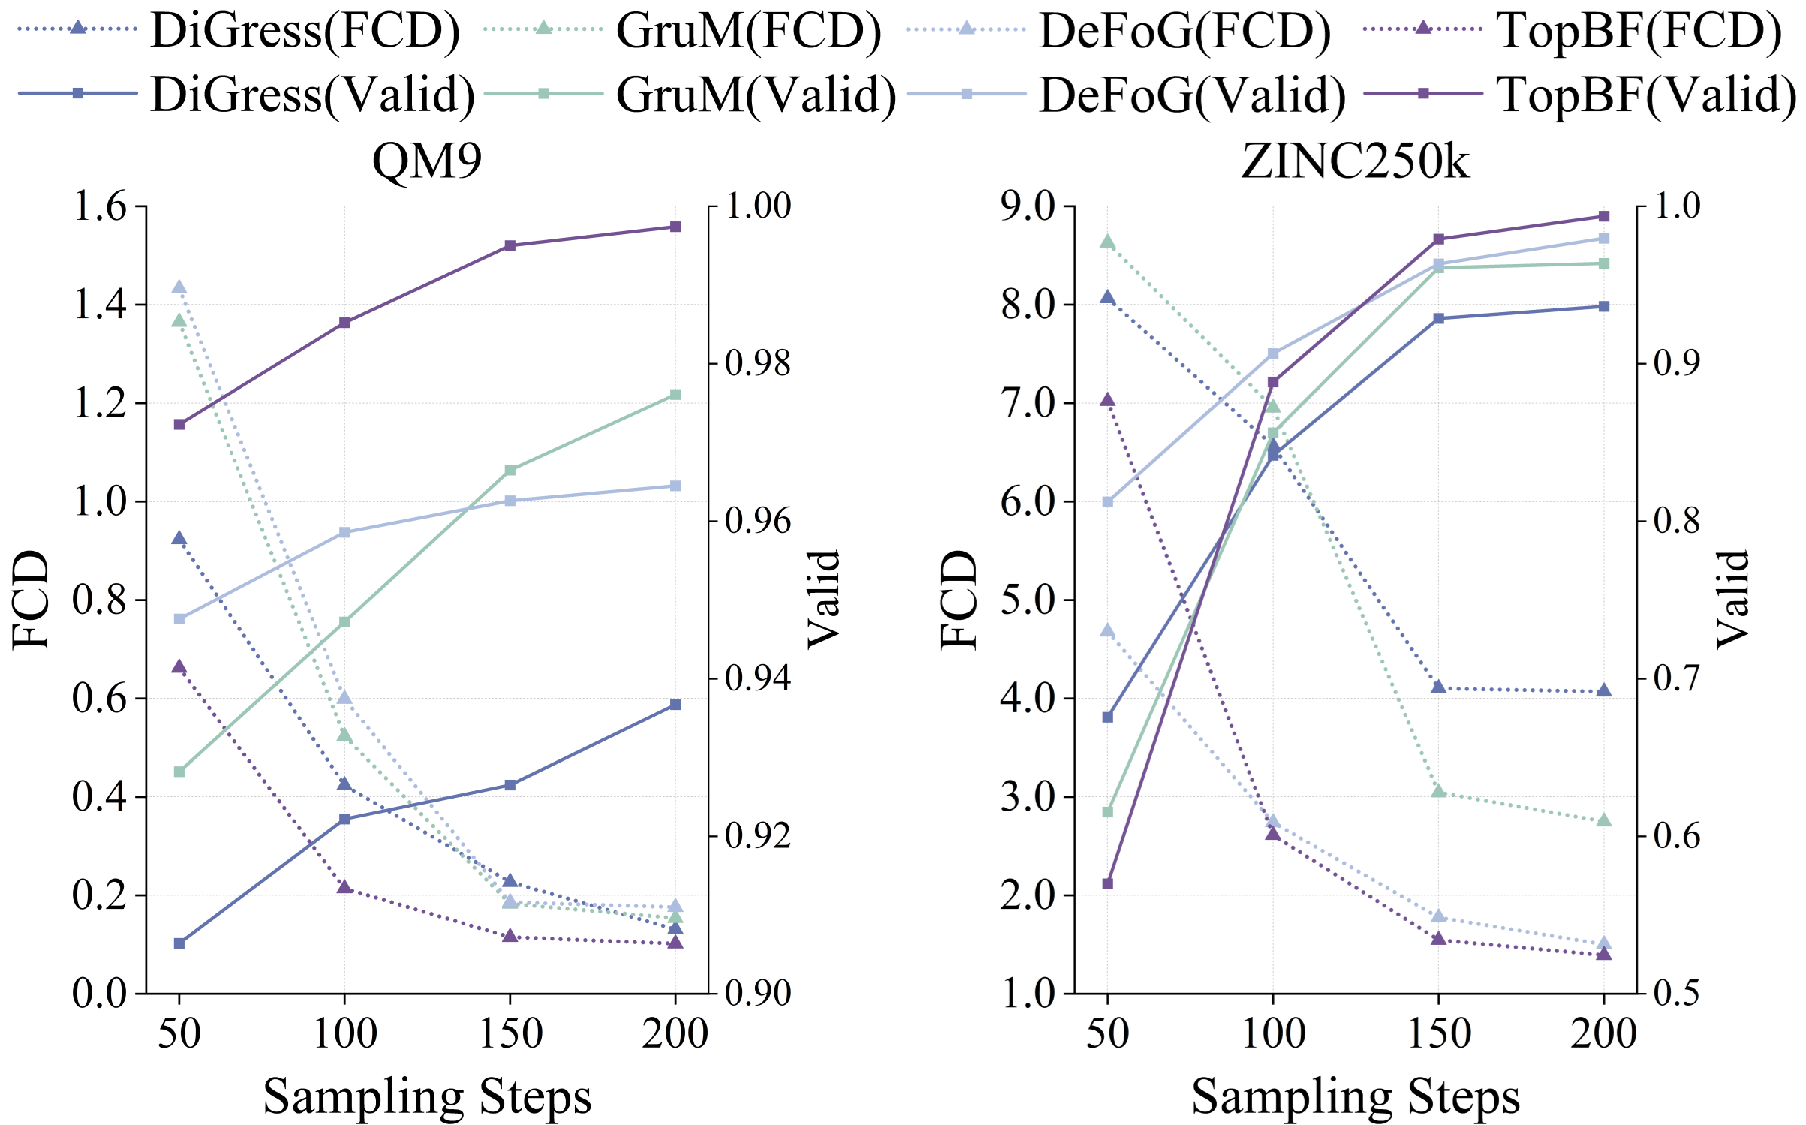
\includegraphics[width=1.\linewidth]{sampling.pdf}
    \caption{Sampling efficiency comparison between TopBF and baselines on QM9 and ZINC250k datasets.}
    \label{fig:sampling}
\end{figure}


\section{Results}
% We conduct a comprehensive evaluation of TopBF on two standard molecular graph generation benchmarks: QM9 and ZINC250k. Additionally, we compare the sampling effiency of TopBF against representative baselines.

% We evaluate TopBF on two standard molecular graph generation benchmarks, QM9 and ZINC250k, and further examine its controllability, sampling efficiency, and the contribution of the proposed QW coupling. 
% Unless otherwise stated, all comparisons follow the protocol described in Section~\ref{sec:experiments}.


\subsection{Baselines}
We compare our model against several excellent baselines in MGG. 
EDP-GNN \cite{niu2020permutation} models graphs with a permutation invariant approach. 
GDSS \cite{jo2022score} is a score-based diffusion model. 
DiGress \cite{vignac2023digress} generates graphs using a discrete diffusion process. 
LGD \cite{zhou2024unifying} generates and predicts all-level graphs via latent diffusion.
GruM \cite{jo2024graph} models the generative process as a mixture of endpoint-conditioned diffusion.
DeFoG \cite{qinmadeira2024defog} using a discrete flow matching framework that defines continuous-time probability paths over categorical attributes.
SID \cite{boget2025simple} assumes conditional independence between intermediate states to simplify discrete diffusion.


\subsection{Molecular Graph Generation}
% In our experiments, TopBF demonstrates superior performance for most metrics on both QM9 and ZINC250k, as shown in Table~\ref{tab:1}, outperforming previous flow-based, flow matching, and diffusion models. Specifically, overall leading on FCD and NSPDK indicate the molecules generated by TopBF closely align with the distributions of the relevant molecular datasets. Furthermore, the highest score on uniqueness manifests the best diversity performance and exploration capability during generation, which further highlights the deficiency of the methods treating training objective as a regression task. Since all methods attain 100\% validity after molecular correction, recent methods including TopBF meet industrial requirements. Additionally, Table~\ref{tab:1} reveals that TopBF achieves superior effects with significantly fewer sampling steps. We also present randomly selected molecular samples in Appendix~\ref{app:vis} for visualization. 
% % This compelling evidence highlights the effectiveness of our work, facilitating rapid generation of higher-fidelity and more diverse molecular graphs.

Table~\ref{tab:1} summarizes the results on QM9 and ZINC250k. TopBF achieves the best or tied-best performance on most metrics with only $200$ sampling steps, compared with $500$ or $1000$ for major diffusion and flow baselines.

On QM9, TopBF achieves the best validity ($99.74\%$), uniqueness ($99.27$), and FCD ($0.093$), while tying for second on NSPDK ($0.0002$). These gains indicate improved distribution matching without sacrificing diversity.

On ZINC250k, TopBF attains perfect uniqueness ($100.00$), the best FCD ($1.392$), and best NSPDK ($0.0008$), with $99.37\%$ validity. It improves FCD over DeFoG ($1.425$) with fewer sampling steps and substantially outperforms SID in FCD ($2.010$), despite slightly lower validity ($99.50\%$ for SID). Overall, TopBF provides a strong balance of validity, diversity, distributional fidelity, and sampling efficiency. Randomly selected molecules are shown in Appendix 7.



\subsection{Conditional Generation}

% We assess the controllability of TopBF on QM9 by conditioning on graph-level properties, following the setting of DiGress \cite{vignac2023digress}. From the QM9 test split we randomly select $100$ molecules, record their dipole moment $\mu$ and HOMO energy, and use each pair $(\mu^\star,\mathrm{HOMO}^\star)$ as a target. For every target we generate $10$ molecules unconditionally and conditionally with PEG guidance, respectively. $\mu$ and HOMO are computed with Psi4 \cite{smith2020psi4} from conformers built with RDKit \footnote{\url{https://www.rdkit.org}}, and mean absolute error (MAE) is reported between the targets and the estimated properties for above three tasks. We also carry out sensitivity analysis on $\lambda$. As shown in Table~\ref{tab:qm9-conditional}, TopBF with PEG guidance consistently yields lower MAE than the unconditional sampler, demonstrating effective property control. PEG with $\lambda=1.0$ performs best, as we infer that $\lambda=0.5$ guides little during sampling and guidance strength with $\lambda=1.5$ invades the original gradient to generate valid molecules, affecting the property values conversely.

% We next examine whether TopBF supports controllable generation on QM9. From the QM9 test split we randomly select $100$ molecules, record their dipole moment $\mu$ and HOMO energy, and use each pair $(\mu^\star,\mathrm{HOMO}^\star)$ as a target. For every target we generate $10$ molecules unconditionally and conditionally with PEG guidance, respectively. $\mu$ and HOMO are computed with Psi4 \cite{smith2020psi4} from conformers built with RDKit \footnote{\url{https://www.rdkit.org}}, and mean absolute error (MAE) is reported between the targets and the estimated properties for above three tasks. As shown in Table~\ref{tab:qm9-conditional}, PEG guidance consistently reduces the MAE relative to unconditional sampling for all three tasks, namely dipole moment $\mu$, HOMO energy, and joint conditioning on both properties. The best performance is obtained at $\lambda=1.0$, where the MAE decreases from $1.69$ to $0.63$ for $\mu$, from $0.96$ to $0.51$ for HOMO, and from $1.73$ to $0.77$ for joint conditioning. These results show that TopBF can be steered effectively towards desired molecular properties without retraining the base generative model. We also observe a clear dependence on the guidance strength: $\lambda=0.5$ improves control but remains conservative, whereas $\lambda=1.5$ weakens performance relative to $\lambda=1.0$, indicating that overly strong guidance may disturb the original sampling trajectory.

We evaluate controllable generation on QM9 using $100$ test molecules, taking each molecule's dipole moment $\mu$ and HOMO energy as targets. For each target, we generate $10$ molecules with and without PEG guidance. Properties are computed with Psi4 \cite{smith2020psi4} from RDKit conformers \footnote{\url{https://www.rdkit.org}}, and mean absolute error (MAE) is reported for $\mu$, HOMO, and joint conditioning. As shown in Table~\ref{tab:qm9-conditional}, PEG consistently reduces MAE, with $\lambda=1.0$ performing best: $1.69\!\to\!0.63$ for $\mu$, $0.96\!\to\!0.51$ for HOMO, and $1.73\!\to\!0.77$ jointly. Thus, TopBF supports effective property control without retraining. Moreover, $\lambda=0.5$ improves control but remains conservative, whereas $\lambda=1.5$ weakens performance relative to $\lambda=1.0$, indicating that overly strong guidance may disturb the original sampling trajectory.




\subsection{Sampling Efficiency and Effect}
% We conduct a sampling efficiency experiment to compare the sampling velocity against representative baselines. As manifested in Figure~\ref{fig:sampling}, our method exhibits exceptional performance during initial 100 steps. Scores could be further improved if sampling with steps longer than 200. However, we choose 200 steps as the best accuracy-efficiency trade-off. This characteristic renders TopBF well-suited for generating high-quality molecular samples while maintaining competitive in inference time.

Figure~\ref{fig:sampling} compares TopBF with representative baselines under different sampling budgets. TopBF reaches a strong performance within the first $100$ steps and continues to improve with additional steps, although the gains become more gradual afterwards. Based on this trend, we use $200$ steps as the default setting, which provides a favorable balance between generation quality and computational cost. Under this budget, TopBF remains competitive with, and in several cases superior to, methods that require considerably longer trajectories. This behaviour is consistent with the Bayesian flow formulation, where the model directly evolves distribution parameters and produces useful categorical confidence early in the sampling process.




\subsection{Ablation on Quasi-Wasserstein Coupling}
\label{sec:ablation_qw}

% We further conduct an ablation study to isolate the effect of the proposed QW transport coupling on atom types and bond types. All variants share the same architecture, training schedule, and sampling steps, differing only in whether the topology-aware transport objective is activated on atoms and/or bonds. As reported in Table~\ref{tab:ablation_qw}, applying QW to both atoms and bonds achieves the best overall performance. Moreover, the two partial variants reveal complementary behaviors, where enabling QW on atoms mainly enhances distributional fidelity reflected by FCD, while enabling QW on bonds primarily strengthens validity and graph-structural alignment reflected by NSPDK. Removing QW leads to a uniform degradation, indicating that topology-aware transport coupling provides an effective structural learning signal beyond CDF-aligned Bayesian flow objective with the default $L_2$ regularization, and that jointly coupling atoms and bonds yields the most reliable gains.

Table~\ref{tab:ablation_qw} reports the ablation study on the proposed QW transport coupling. Removing QW entirely leads to a clear degradation on both datasets. On QM9, validity drops from $99.74\%$ to $98.63\%$ and FCD worsens from $0.093$ to $0.143$. On ZINC250k, the effect is more pronounced, with validity decreasing from $99.37\%$ to $94.75\%$ and FCD deteriorating from $1.392$ to $3.959$. This indicates that the topology-aware transport objective contributes substantially beyond the base Bayesian flow loss.

The partial ablations further suggest that atom-level and bond-level coupling play different roles. Enabling QW on atoms mainly improves distributional fidelity, reflected by the strongest FCD on ZINC250k ($1.347$) and high uniqueness on both datasets. In contrast, enabling QW on bonds mainly benefits structural correctness, giving the best validity on QM9 ($99.81\%$) and strong NSPDK on both datasets. When both components are used together, TopBF achieves the best overall balance across validity, uniqueness, FCD, and NSPDK. This supports the design choice of jointly coupling node and edge variables in the transport objective.


\section{Conclusion}
\label{sec:conclusion}

In this paper, we introduce \textbf{TopBF}, a transport-coupled Bayesian Flow framework for molecular graph generation. TopBF operates in continuous parameter distributions and employs a CDF-based output channel to directly compute category probabilities, aligning the training objective with the discrete discretization used during sampling procedure, rather than fitting arbitrary continuous embeddings. To further inject topology awareness without breaking closed-form Bayesian updates, we formulate a Quasi-Wasserstein transport coupling under geodesic costs, encouraging topology-consistent alignment of atom and bond categorical mass on molecular graphs. Empirically, TopBF achieves state-of-the-art results on standard molecular graph generation benchmarks with efficient sampling of the minimum steps.


\section*{Supplementary data}

Supplementary data are available as an attachment. Reproducible code is available at \url{https://github.com/Cello2195/TopBF/tree/main}.

% \section*{Conflict of interest}

% None declared.


\section*{Funding}

This work was supported by 
the Natural Science Foundation of China (No.62476203), 
the Key Project of Traditional Chinese Medicine Joint Fund of Hubei Provincial Natural Science Foundation (No.2025AFD47), 
the Hubei Province Science and Technology Innovation Plan Project (No.2025BCB035), 
the Shenzhen Natural Science Foundation Project (No.JCYJ20250604122534006, 

\noindent JCYJ20230807090211021), 
Guangdong Provincial Natural Science Foundation General Project (No.2025A1515012155). 
Independent Project of Basic Scientific Research Business Fundation of Chinese Academy of Traditional Chinese Medicine (No.ZZ180301).




\bibliographystyle{IEEEtran}
\bibliography{reference}

\end{document}